\documentclass[usenames,dvipsnames,notes]{beamer}
\usepackage{ifthen}
\usepackage{xcolor}
\usepackage{pgfplots}
\usepackage{amsmath}
\usepackage{centernot}
\usepackage{pifont}
\usepackage{tabularx}
\usepackage{makecell}
\usepackage{cuted}
\usepackage{booktabs}
\usepackage{array}
\usepackage{tcolorbox}
\usepackage{subcaption}

\usepackage{pgfpages}
%\setbeameroption{show notes on second screen}


\input ../beamer-style
\input ../std-macros
\input ../macros

\AtBeginSubsection[]
{
    \begin{frame}
        \frametitle{Table of Contents}
        \tableofcontents[currentsection,currentsubsection]
    \end{frame}
}
\parskip=10pt

\title[CSCI-GA.2590]{Grounded Language Understanding}
\author[He He]{He He
}
\institute[NYU]{New York University}
\date{\today}

\begin{document}
\begin{frame}
\titlepage
\end{frame}

\begin{frame}
    {Logistics}
    Plan for the rest of the semester\\
    \begin{itemize}
        \item Next week
            \begin{itemize}
                \item Guest lecture by Victoria Lin\\
                Title: Conversation with Data: Where We Are and What's Next
            \item Writing and presentation, summary and outlook
            \end{itemize}
        \item Final week: project presentations\\
            About 30 groups, 3 min talk + 1 min Q\&A
        \item Deliverables
            \begin{itemize}
                \item HW4: CKY parser, due Dec 8
                \item Project report: due Dec 20 
            \end{itemize}
    \end{itemize}
\end{frame}

\section{Introduction}

\begin{frame}
    {Steven Colbert's conversation with Siri}
    \begin{columns}
        \begin{column}{0.3\textwidth}
            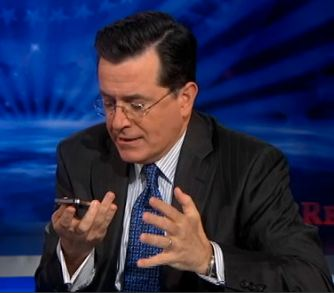
\includegraphics[width=3cm]{figures/colbert-siri}
        \end{column}
        \begin{column}{0.7\textwidth}
            \begin{tabular}{lp{6cm}}
                Colbert: & What am I talking about tonight? \\
                Siri: & I would perfer not to say. \\
                ... & ...\\
                Colbert: & For the love of \textcolor{Green}{God}, the \emph{cameras} are on, give me something?\\
                Siri: & What kind of place are you looking for? \emph{Camera stores} or \textcolor{Green}{churches} \\
                ... & ...\\
                Colbert: & I don't want to search for anything! I want to write the show!\\
                Siri: & Searching the Web for ``search for anything. I want to write the shuffle.''
            \end{tabular}
        \end{column}
    \end{columns}
\end{frame}

\begin{frame}
    {What went wrong?}
    What am I talking about tonight?\\
    \begin{itemize}
        \item Who is ``I''?
        \item When is ``tonight''?
        \item What's the purpose of the talk?
        \item Who's the audience?
    \end{itemize}

    Context is important!\\
    \begin{itemize}
        \item Where are you from? (nation, hometown, school?) 
        \item (Ice or no ice? Coffee or tea? Morning or afternoon?) The latter, please.
        \item Can you pass me the salt?
    \end{itemize}
\end{frame}

\begin{frame}
    {Language and communication}
    \begin{columns}
        \begin{column}{0.4\textwidth}
            \begin{figure}
            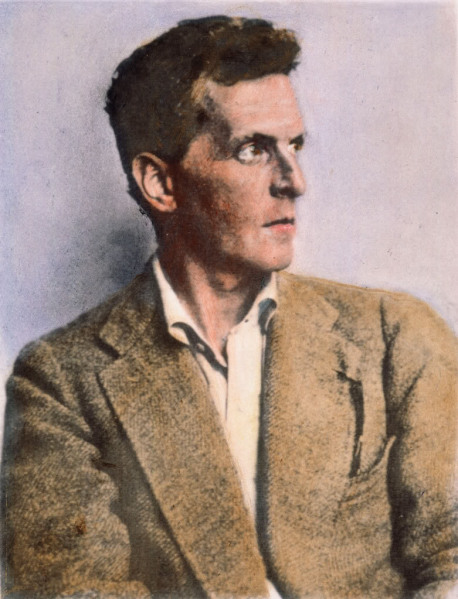
\includegraphics[width=3.5cm]{figures/ludwigwittgenstein}
            \end{figure}
        \end{column}
        \begin{column}{0.6\textwidth}
            Wittgenstein, \textit{Philosophical Investigations}

            \vspace{1em}
            ``For a large class of cases of the employment of the word ‘meaning’---though not for all—this word can be explained in this way: \emph{the meaning of a word is its use in the language}''
            \begin{figure}
            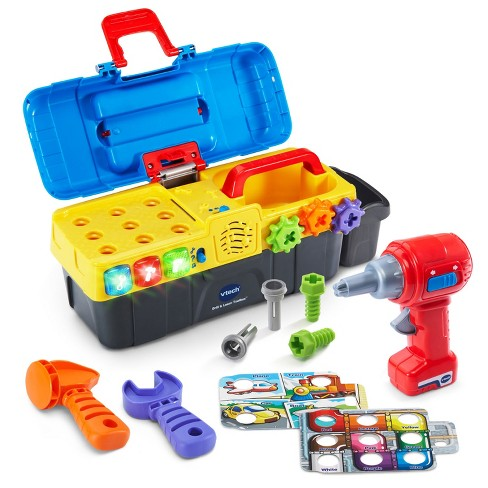
\includegraphics[width=3cm]{figures/tools}
            \end{figure}
        \end{column}
    \end{columns}
\end{frame}

\begin{frame}
    {SHRDLU [Winograd 1972]}
    \begin{columns}
        \begin{column}{0.3\textwidth}
            \begin{figure}
                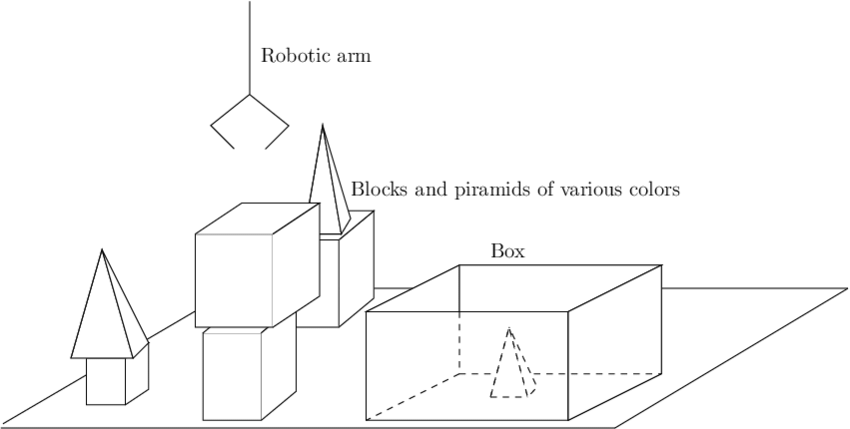
\includegraphics[width=4cm]{figures/shrdlu}
            \end{figure}
        \end{column}
        \begin{column}{0.6\textwidth}
            \begin{tabular}{lp{5cm}}
        Person: & Pick up a big red block.\\
        Computer: & OK.\\
        Person: & Grasp the pyramid.\\
        Computer: & I DON'T UNDERSTAND WHICH PYRAMID YOU MEAN.\\
        ... & ...
    \end{tabular}
        \end{column}
        \end{columns}
        \medskip
        \begin{itemize}
            \item Connect symbols to the world: utterance $\to$ logical form $\to$ action $\to$ response   
            \item Successful but limited to the blocks world
            \item Renewed interest in grounded systems with the success of neural networks 
        \end{itemize}
\end{frame}

\begin{frame}
    {Tasks that involve grounding}

    Describing color \mycite{[MacMahan and Stone, 2015]}
    \vspace{-1em}
    \begin{figure}
        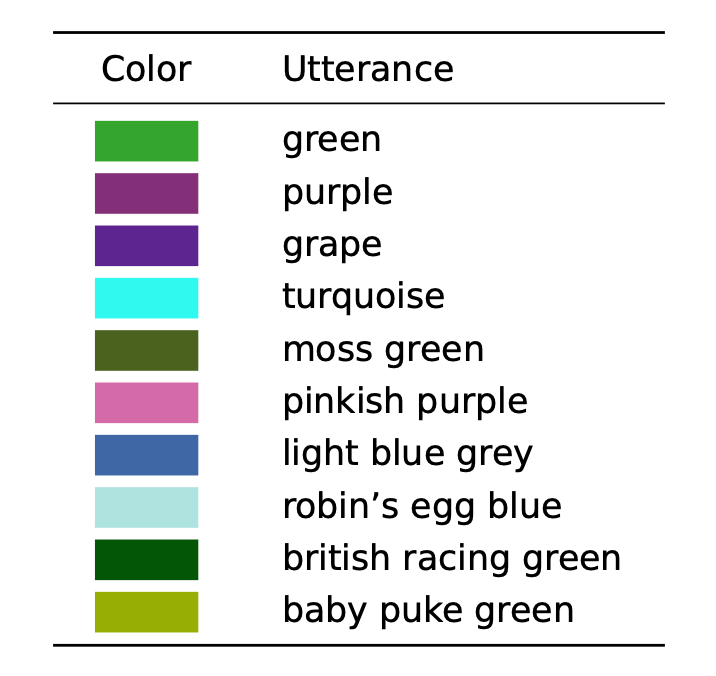
\includegraphics[height=5cm]{figures/color}
        \caption{Example from Chris Potts}
    \end{figure}
\end{frame}

\begin{frame}
    {Tasks that involve grounding}

    Visual question answering \mycite{[Agrawal+ 2015]}
    \vspace{-1em}
    \begin{figure}
        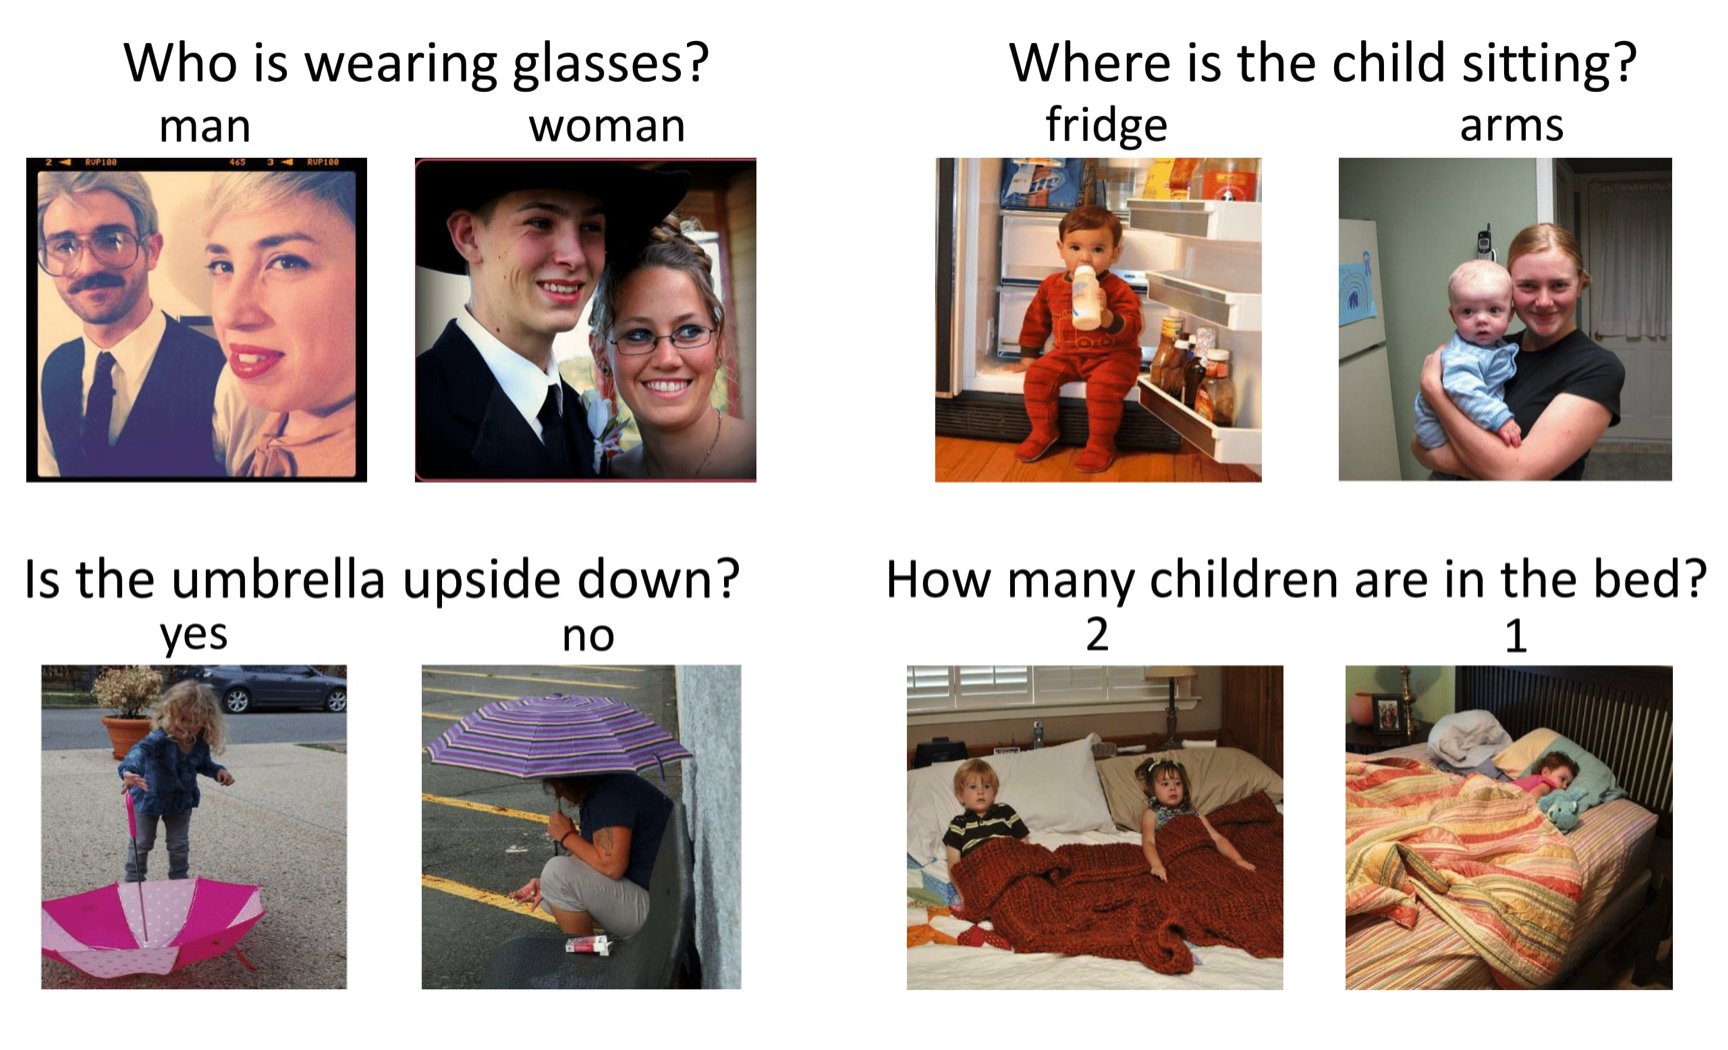
\includegraphics[height=5cm]{figures/vqa}
    \end{figure}
\end{frame}

\begin{frame}
    {Tasks that involve grounding}

    CLEVR: visual reasoning \mycite{[Johnson+ 2015]}
    \vspace{-1em}
    \begin{figure}
        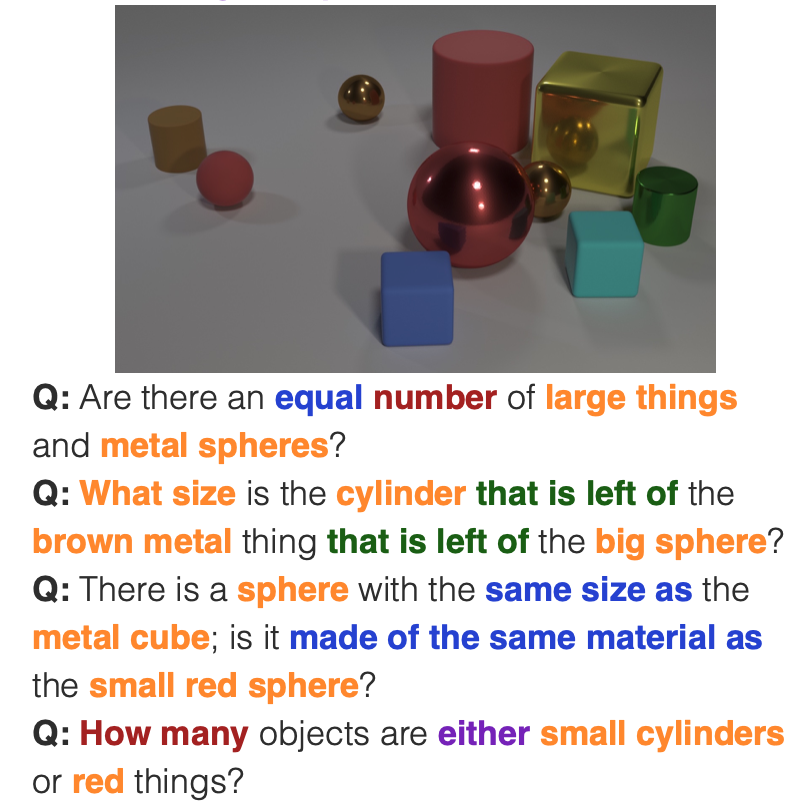
\includegraphics[height=6cm]{figures/clevr}
    \end{figure}
\end{frame}

\begin{frame}
    {Tasks that involve grounding}

    Spatial reasoning \mycite{[Bisk+ 2017]}
    \vspace{-1em}
    \begin{figure}
        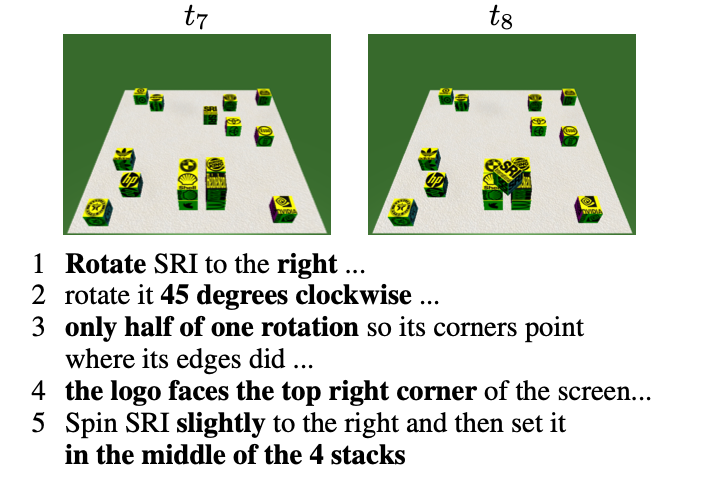
\includegraphics[height=6cm]{figures/spatial}
    \end{figure}
\end{frame}

\begin{frame}
    {Tasks that involve grounding}

    ALFRED: instruction following \mycite{[Shridhar+ 2020]}
    \vspace{-1em}
    \begin{figure}
        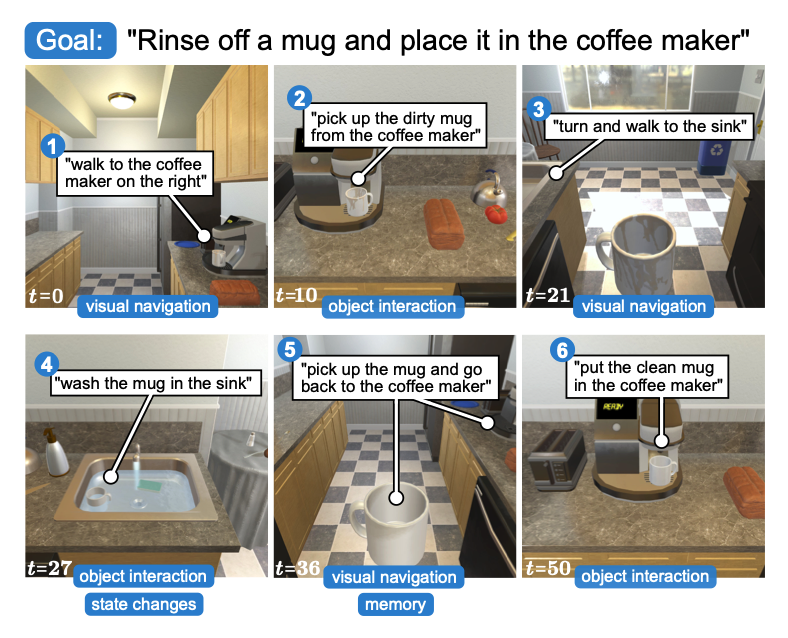
\includegraphics[height=6cm]{figures/alfred}
    \end{figure}

    With real robots, see \mycite{[Chai+ 2018]}.
\end{frame}

\begin{frame}
    {Tasks that involve grounding}

    Empathetic dialogue \mycite{[Rashkin+ 2020]}
    \vspace{-1em}
    \begin{figure}
        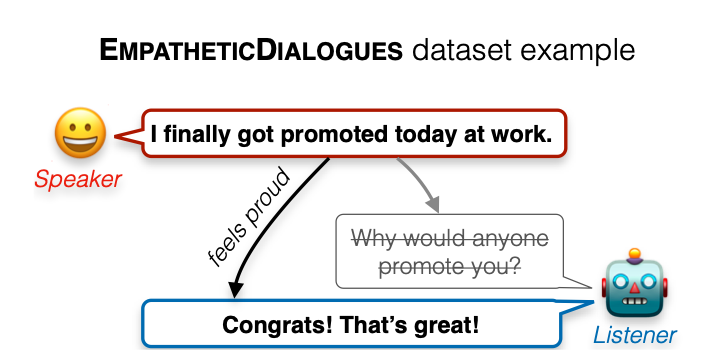
\includegraphics[height=5cm]{figures/empathetic}
    \end{figure}
\end{frame}

\begin{frame}
    {Tasks that involve grounding}
    Winograd schema challenge \mycite{[Winograd 1972, Levesque 2011, Davis+ 2016]}

    \textcolor{blue}{Jim} yelled at Kevin because \textcolor{blue}{he} was so upset.\\
    Jim comforted \textcolor{blue}{Kevin} because \textcolor{blue}{he} was so upset.

    \bigskip
    \textcolor{blue}{The customer} walked into the bank and stabbed one of the tellers. \textcolor{blue}{He} was immediately taken to the police station.\\
    The customer walked into the bank and stabbed one of \textcolor{blue}{the tellers}. \textcolor{blue}{He} was immediately taken to the hospital.

    \bigskip
    Ground in social, physical context
\end{frame}

\begin{frame}
    {Summary}
    Connects language (symbols) to the world\\
    \begin{itemize}
        \item \emph{Perception}: vision, audio
        \item \emph{Action}: navigation, interaction
        \item \emph{Society}: commonsense, empathy
    \end{itemize}

    model $\to$ agent\\
    \begin{itemize}
        \item Multimodal: full perception of the world
        \item Interactive: actively learn about the world 
        \item Multi-agent: consider other agents in the world 
    \end{itemize}
\end{frame}

\section{Key frameworks for language grounding}
\begin{frame}
    {Useful frameworks for thinking about grounding problems}
    Multimodal: mapping between different types of signals\\
    \begin{itemize}
        \item Neural architectures that encode different signals in the same space
    \end{itemize}

    Interactive: take actions and receive feedbacks\\
    \begin{itemize}
        \item Reinforcement learning: learning from trial and error
    \end{itemize}

    Multi-agent: 
            model other agents' goals and contexts\\
    \begin{itemize}
        \item Speakers: generate language given the world 
        \item Listeners: interpret language in the world 
        \item The rational speech act model: reason about each other
    \end{itemize}
\end{frame}

\subsection{Multimodal representation}
\begin{frame}
    {Basic multimodal architecture}
    Key components:\\
    \begin{enumerate}
        \item Encoders: embed different signals separately
        \item Fusion: create interaction among different embeddings 
        \item Decoder: classification, generation etc.
    \end{enumerate}
    \vspace{-1em}

    \begin{figure}
        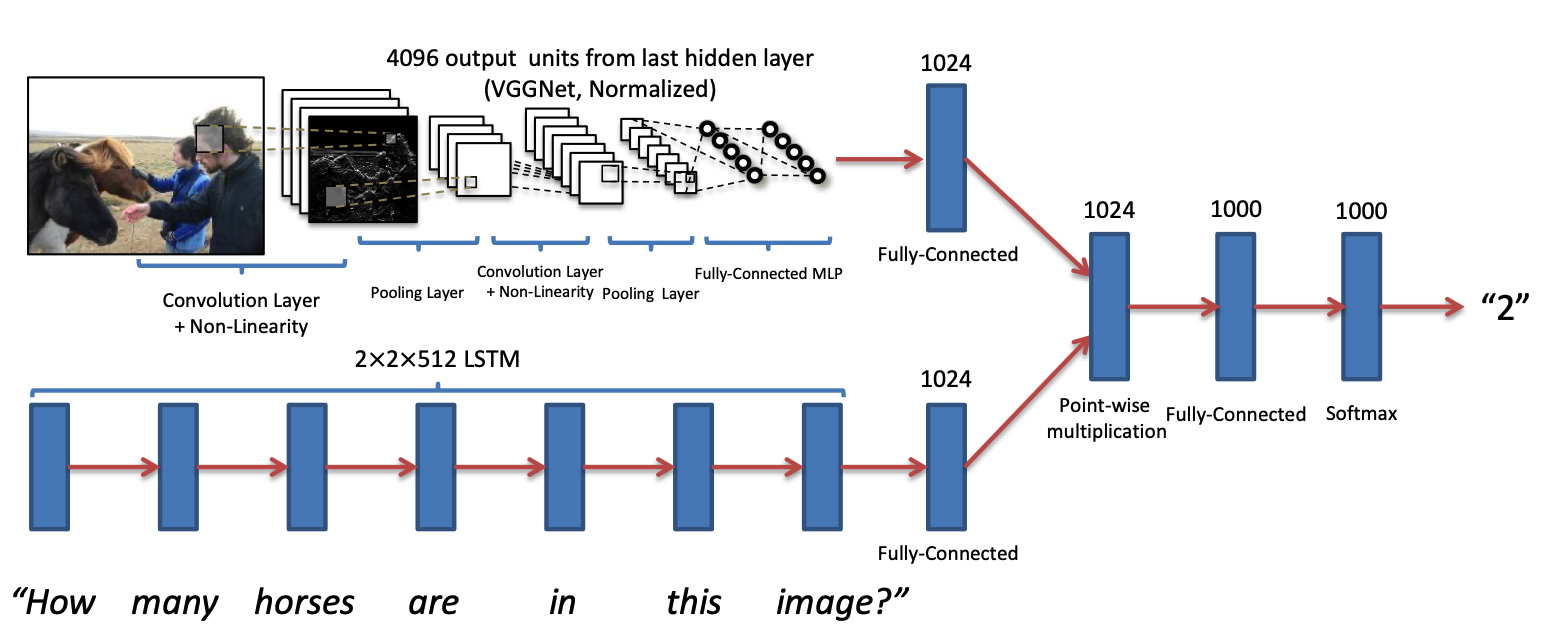
\includegraphics[height=4cm]{figures/vqa-model}
        \caption{[Agrawal+ 2016]}
    \end{figure}
\end{frame}

\begin{frame}
    {Attention over image}
    Similar to text QA, we want to interact different parts in the text and the image.

    What are ``words'' in images?

    \begin{figure}
        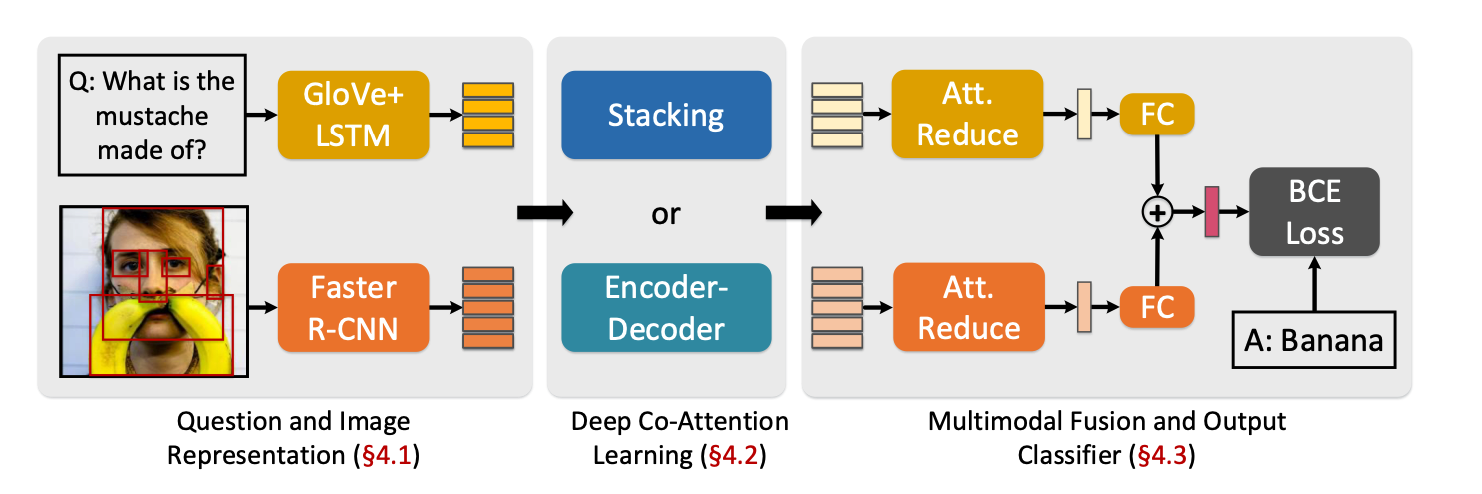
\includegraphics[height=4cm]{figures/vqa-attention}
        \caption{[Yu+ 2019]}
    \end{figure}
\end{frame}

\begin{frame}
    {Neural module networks}
    Visual reasoning $\iff$ semantic parsing
    \begin{figure}
        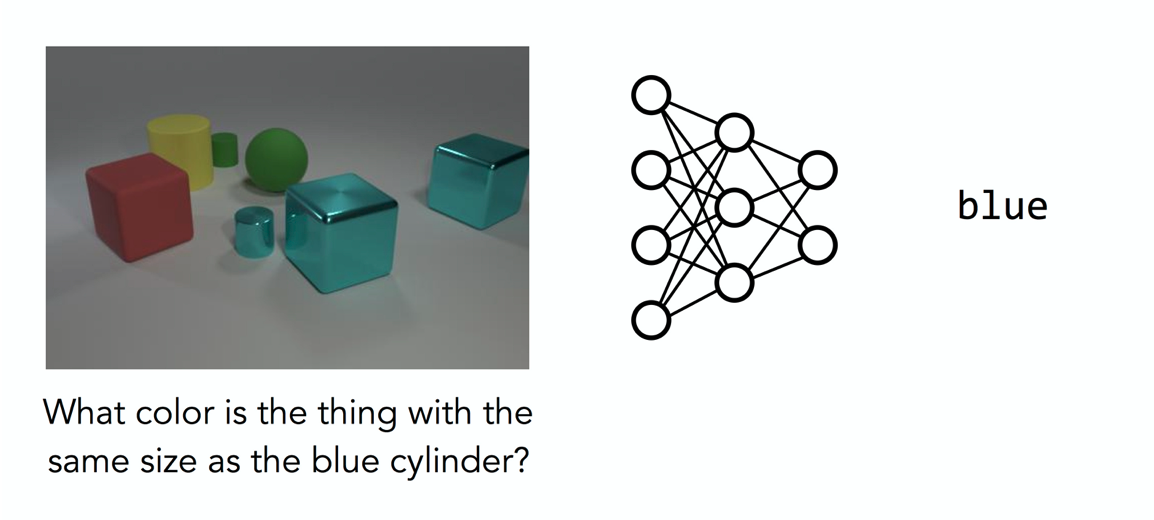
\includegraphics[height=4cm]{figures/nmn-ex}
    \end{figure}
    $$
    \texttt{color}(
    \lambda x.\texttt{equal}(
    \texttt{size}(x),
    \texttt{size}(\lambda y.\texttt{blue}(y) \land \texttt{cylinder}(y))
    )
    )
    $$
    How do we execute the logical form on an image?
\end{frame}

\begin{frame}
    {Neural module networks}
    \begin{tabular}{lll}
        Text& $\texttt{capital}(x)$ & database lookup \\
        Image& $\texttt{color}(x)$ & learned function $f_{\text{color}}(x, \text{image})$
    \end{tabular}

    Share modules (``predicates''/functions) across examples

    \vspace{-1em}
    \begin{figure}
        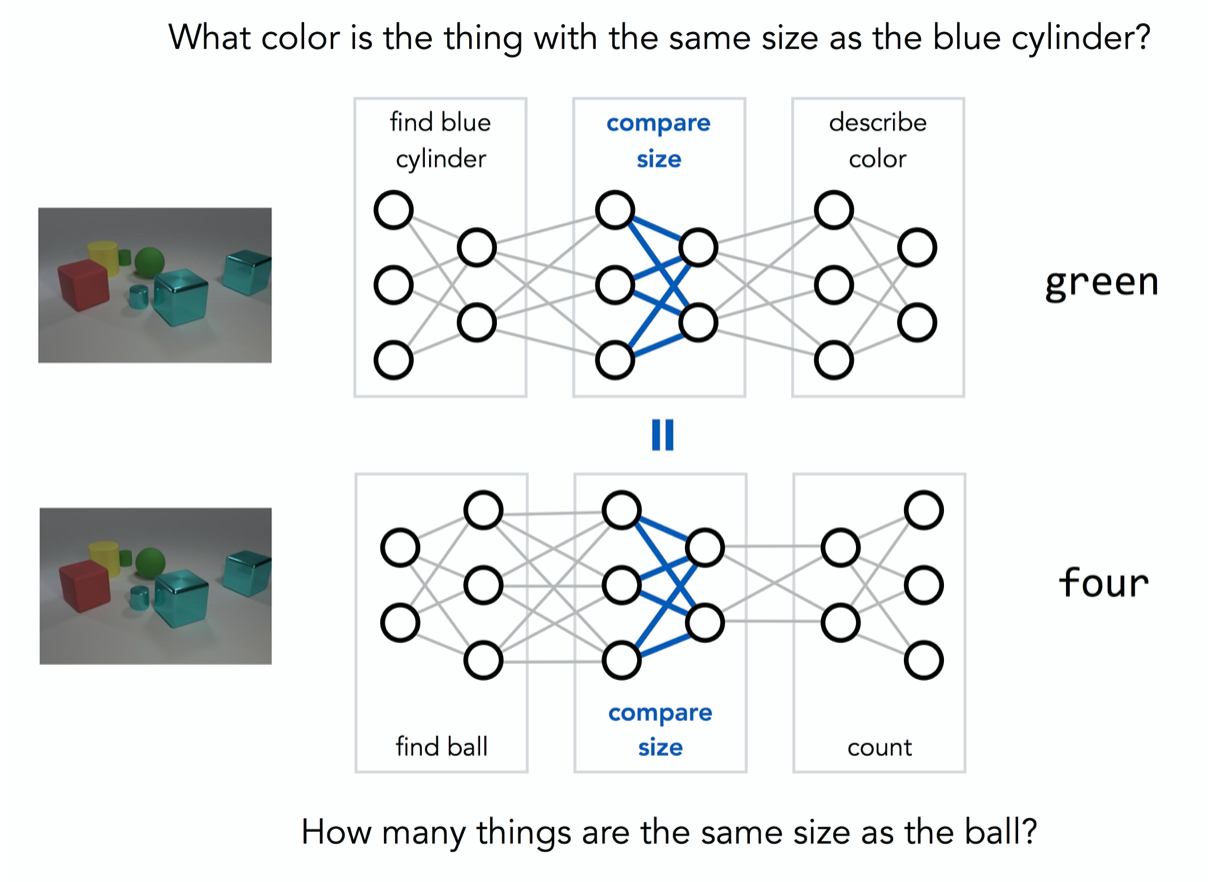
\includegraphics[height=5cm]{figures/nmn-ex2}
    \end{figure}
\end{frame}

\begin{frame}
    {Neural module networks}
    Compose modules:\\
    \begin{enumerate}
        \item Universal representation: dependency parse (objects and attributes, events and participants etc.)
        \item Composition of modules (e.g. $\texttt{color}(x)$, $\texttt{what}(\texttt{fly})$)
            \begin{itemize}
                \item Rule-based mapping (restricted domains) 
                \item Model as a latent variable
                \item Obtain human annotation
            \end{itemize}
    \end{enumerate}

    \vspace{-1em}
    \begin{figure}
        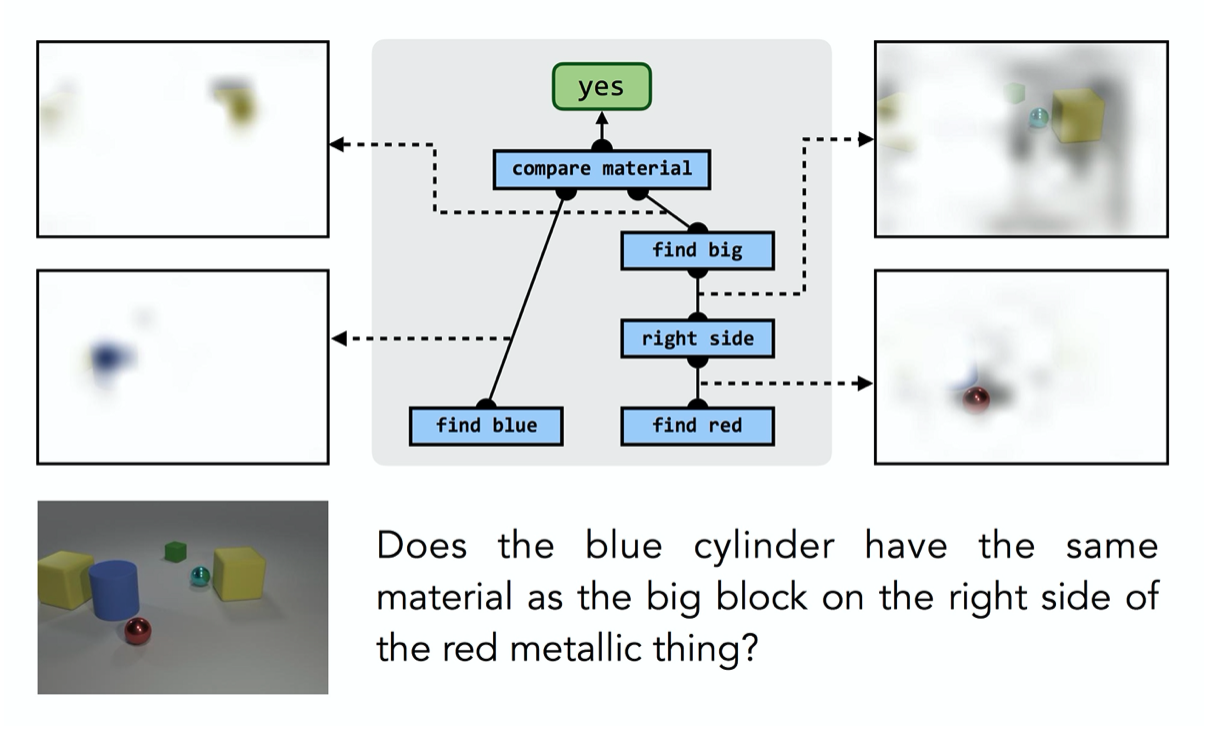
\includegraphics[height=3.5cm]{figures/nmn-ex3}
        \caption{[Andreas+ 2016]}
    \end{figure}
    \vspace{-1em}
\end{frame}

\begin{frame}
    {Multimodal pre-training}
    Data: image caption, VQA \\
    Self-supervision: masked LM, matching between image/text

    \vspace{-1em}
    \begin{figure}
        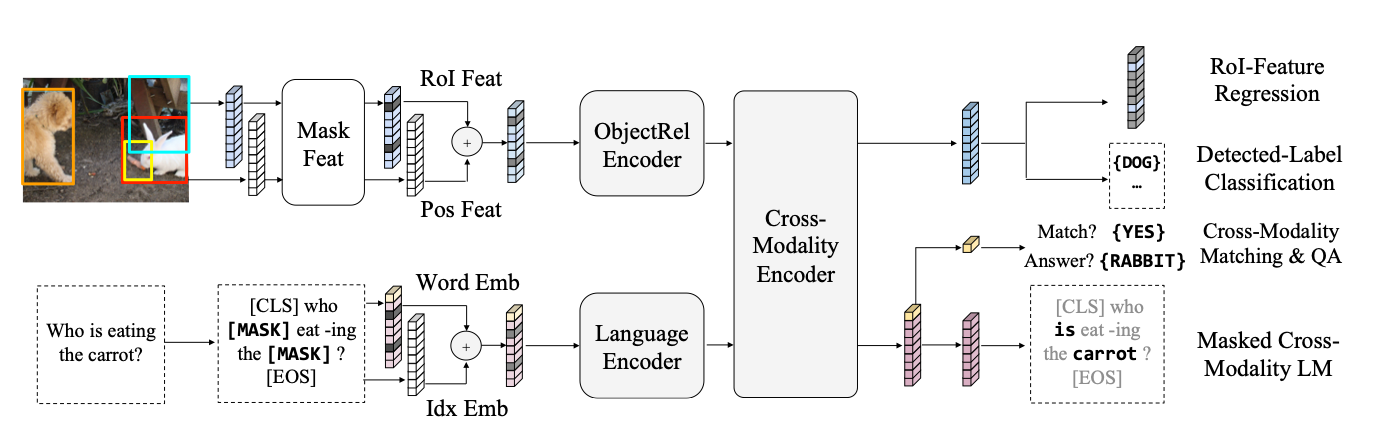
\includegraphics[height=3.5cm]{figures/lxmert}
        \caption{[Tan and Bansal 2019]}
    \end{figure}
\end{frame}

\subsection{Reinforcement learning}
\begin{frame}
    {Learning through interaction}
    \begin{columns}
        \begin{column}{0.4\textwidth}
    \begin{figure}
        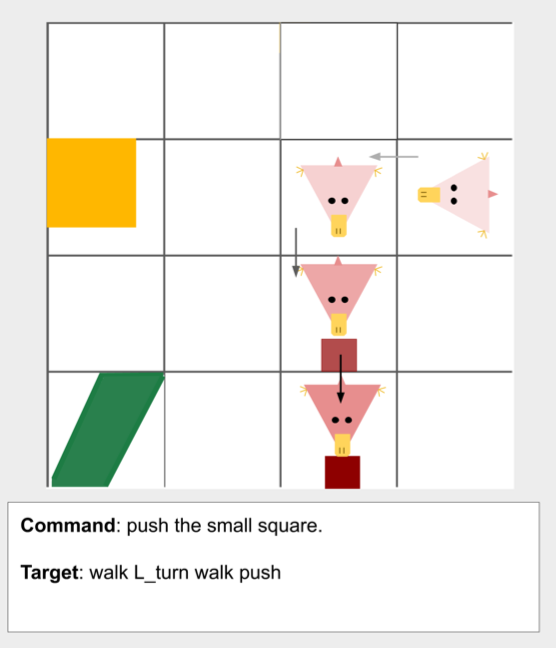
\includegraphics[height=3.5cm]{figures/instruction}
        \caption{[Ruis+ 2020]}
    \end{figure}
        \end{column}
        \begin{column}{0.6\textwidth}
    A trial-and-error strategy:\\
    \begin{itemize}
        \item Agent: Try out random actions in the world 
        \item World: reward agent when goals are achieved
    \end{itemize}
    How to learn from experience?
        \end{column}
    \end{columns}
\end{frame}

\begin{frame}
    {Markov decision process (MDP)}
    \begin{figure}
        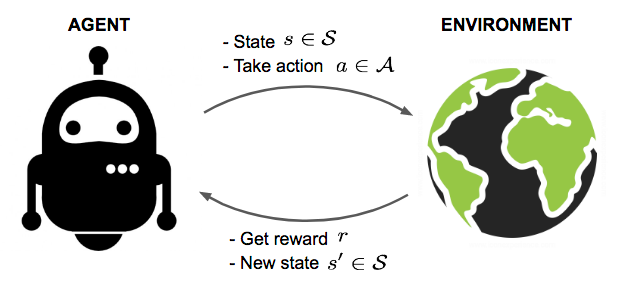
\includegraphics[height=3cm]{figures/rl}
        %\caption{Agent interacts with the environment}
    \end{figure}
    \vspace{-2em}
    \begin{itemize}
        \item At time step $t$, the agent is in \textbf{state} $s_t\in\sS$.
        \item It takes an \textbf{action} $a_t\in\sA$ and transitions to state $s_{t+1}$ with probability $\BP(s_{t+1}=s'\mid s_t=s, a_t=a)$.
        \item The agent receives an immediate \textbf{reward} $r(s, s', a)$.
    \end{itemize}
    \header{Goal}: learn a \textbf{policy} $\pi\colon \sS \to \sA$ that maximizes the expected \textbf{return}
    $$
    \BE\pb{\sum_{t=0}^\infty r(s_t, s_{t+1}, a_t)} \quad \text{ where } a_t\sim\pi(s_t) 
    $$
\end{frame}

\begin{frame}
    {}
    \begin{figure}
        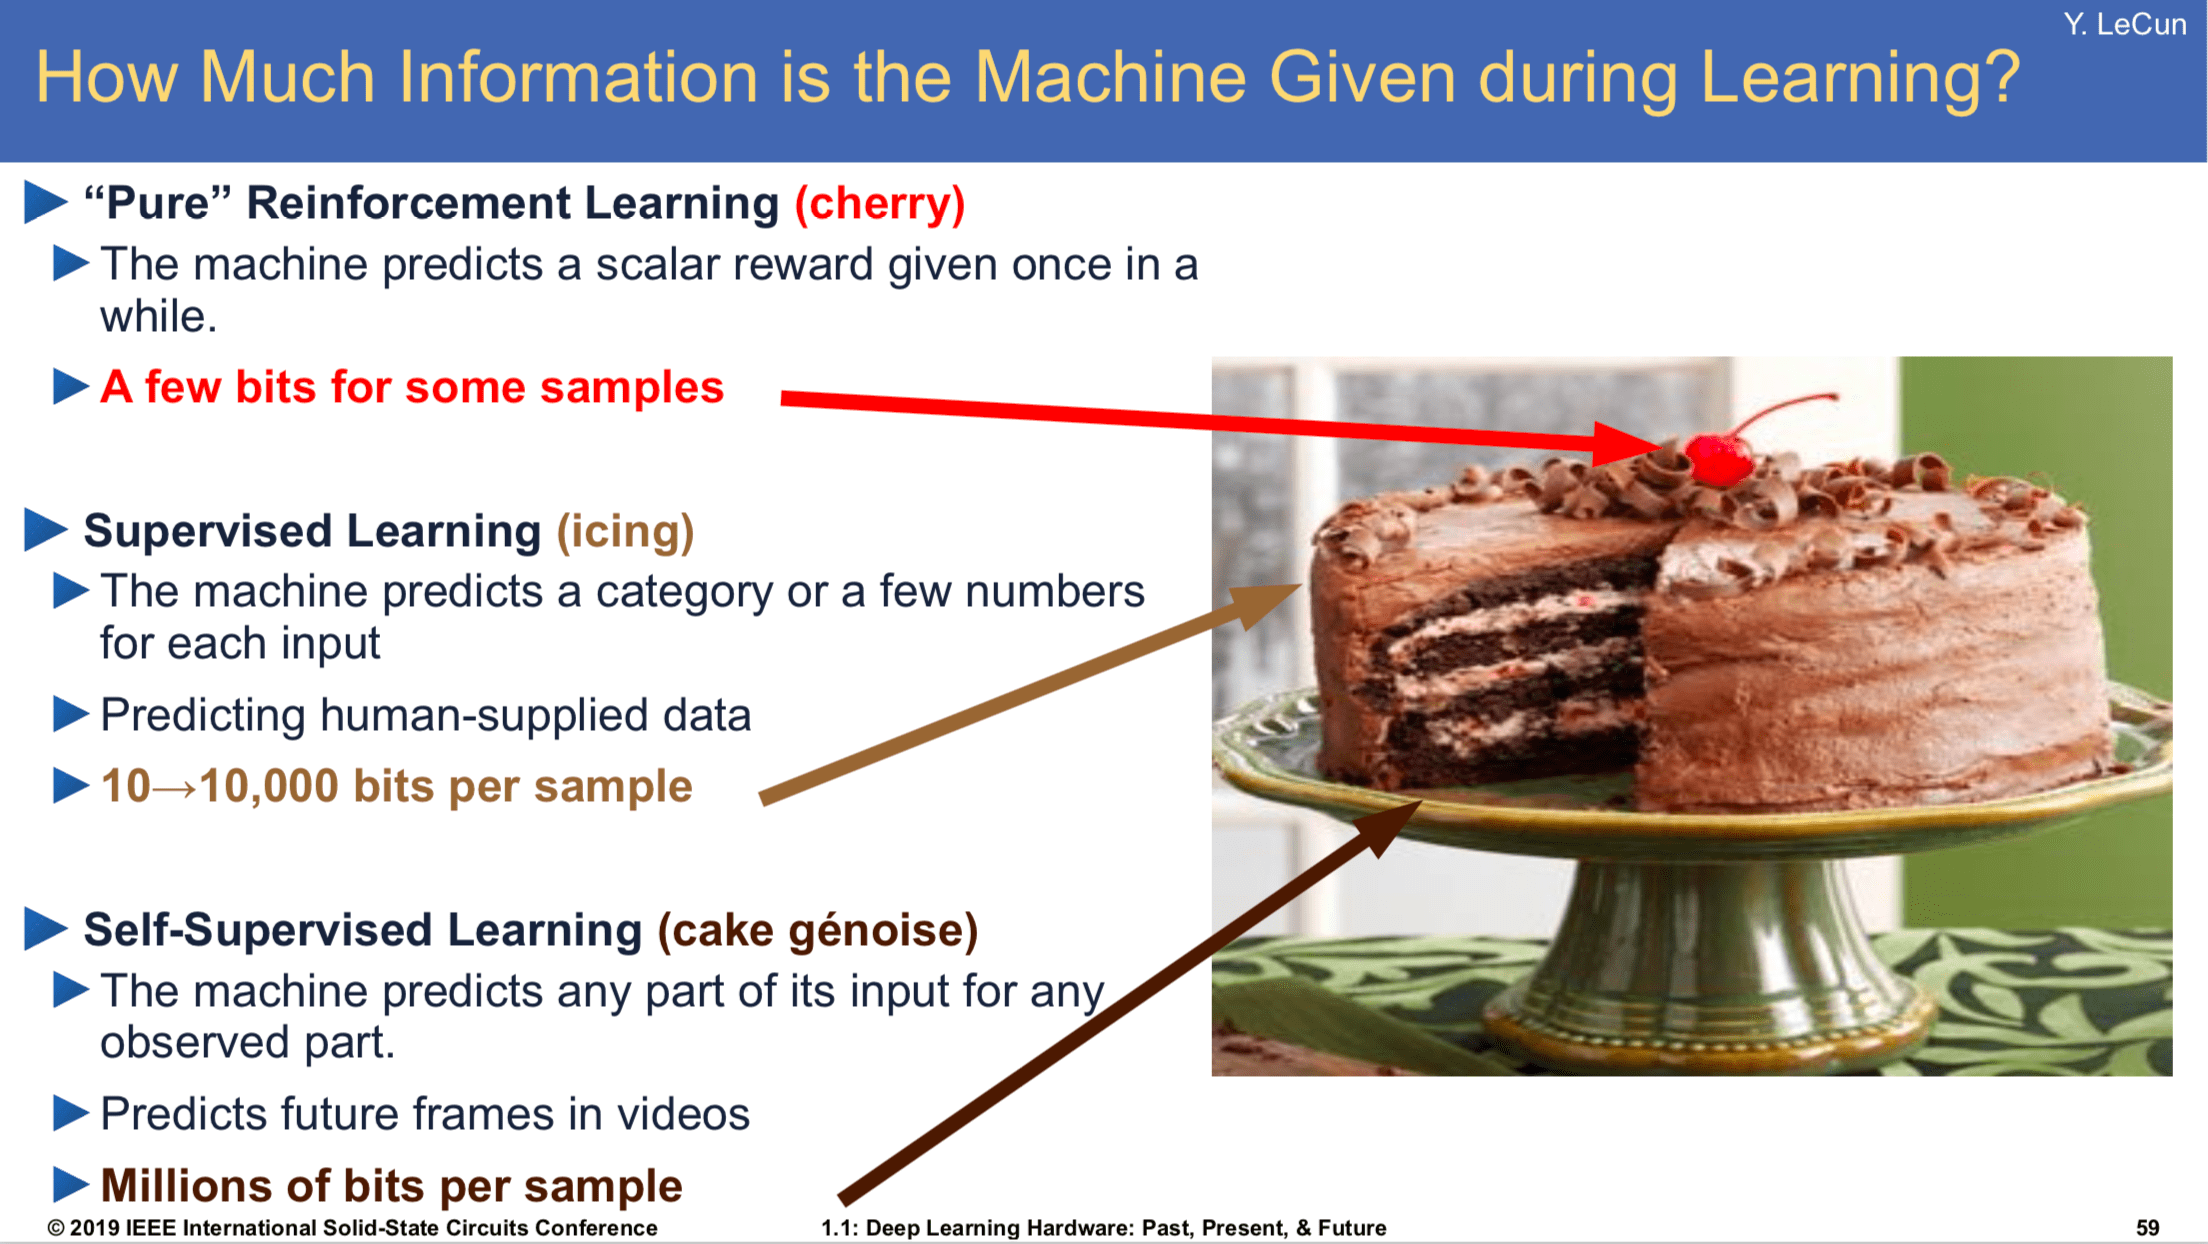
\includegraphics[height=6cm]{figures/yann-rl}
    \end{figure}
    ``If intelligence is a cake, the bulk of the cake is unsupervised learning, the icing on the cake is supervised learning, and the cherry on the cake is reinforcement learning (RL).''---Yann Lecun

\end{frame}

\begin{frame}
    {Challenges in reinforcement learning}
    \begin{columns}
        \begin{column}{.4\textwidth}
    \begin{figure}
        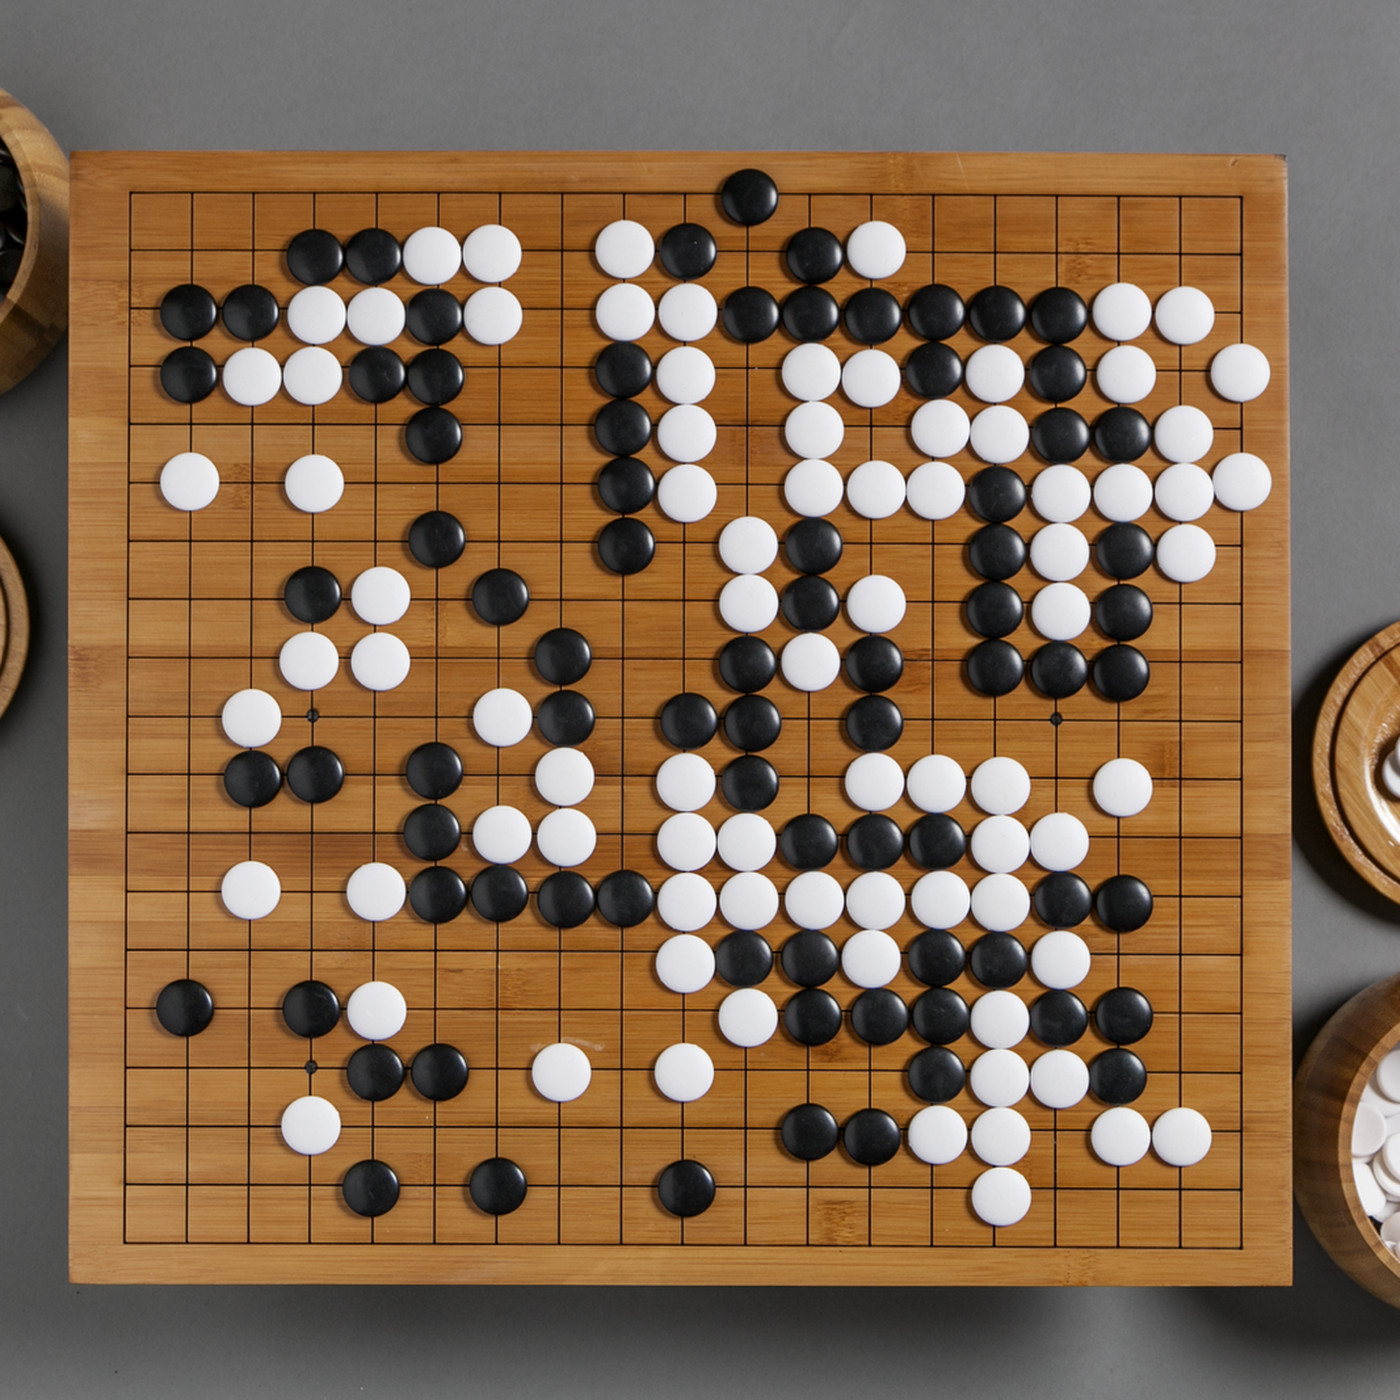
\includegraphics[height=3cm]{figures/go}
    \end{figure}
        \end{column}
        \begin{column}{.6\textwidth}
    \begin{itemize}
        \item \emph{Delayed reward}: which actions are responsible for the reward/penalty?
        \item \emph{Incomplete information}: exploration vs exploitation
        \item Real world RL (education, healthcare, self-driving): expensive exploration
    \end{itemize}
        \end{column}
    \end{columns}
    \bigskip
    \begin{itemize}
        \item Extremely flexible framework
        \item Challenging to do RL from scratch (often needs to pre-train by SL)
    \end{itemize}
\end{frame}

\begin{frame}
    {Example with a simulator}
    \begin{columns}
        \begin{column}{0.4\textwidth}
    \begin{figure}
        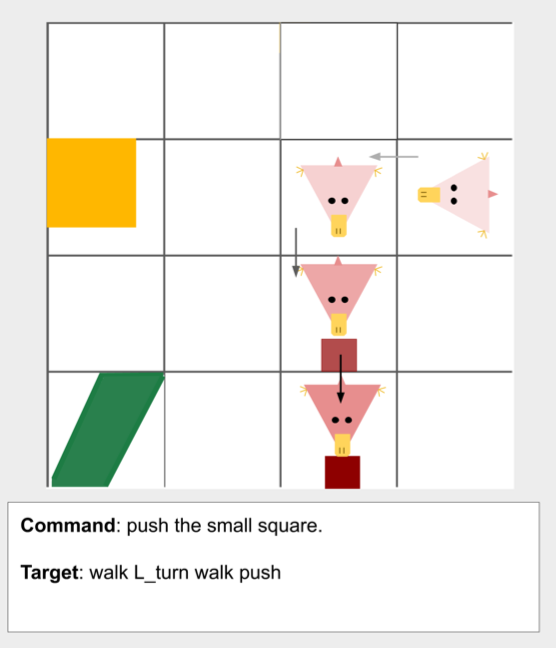
\includegraphics[height=3.5cm]{figures/instruction}
        \caption{[Ruis+ 2020]}
    \end{figure}
        \end{column}

        \begin{column}{0.6\textwidth}
            RL formulation:\\
    \begin{itemize}
        \item Action: walk, turn-L/R, push etc.
        \item What is the state? 
        \item Reward: 1 if the task is completed and 0 otherwise
    \end{itemize}
        \end{column}
    \end{columns}
    Want to learn:\\
    \begin{itemize}
        \item What is a ``square''/``circle''/...?
        \item What is ``small''/``big''/...?
        \item What is ``red''/``green''/``yellow''/...?
    \end{itemize}
\end{frame}

\begin{frame}
    {Policy}
    A typical model for instruction following
    \vspace{-1em}
    \begin{figure}
        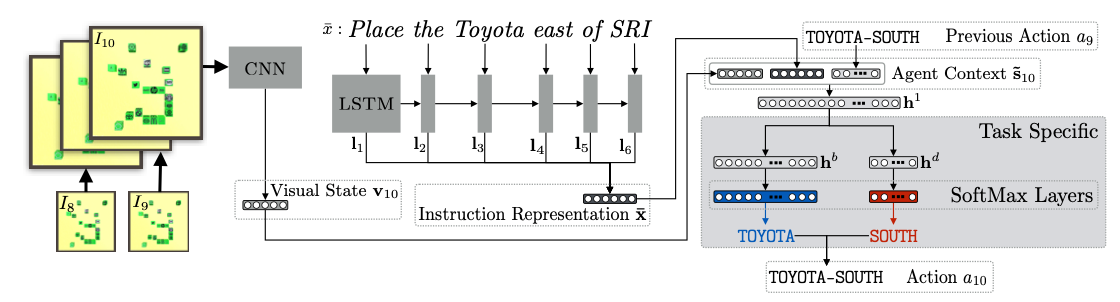
\includegraphics[height=3cm]{figures/policy}
        \caption{[Misra+ 2017]}
    \end{figure}
    \vspace{-1em}
    \begin{itemize}
        \item (visual input, textual instruction) $\to$ action
        \item Stochastic policy:
            $\pi_\theta(a\mid s)=p_\theta(a\mid s)$
        \item Parametrization: multimodal networks.
        \item May need to add history observation into the state.
    \end{itemize}
\end{frame}

\begin{frame}
    {Learning}
    Policy gradient methods:
    directly learn $\pi$ parametrized by $\theta$
    to maximize the expected return
            $$
            \nabla_\theta J(\theta) = \frac{1}{N}\sum_{i=1}^N
            \BE\pb{\nabla_\theta\log\pi_\theta(a\mid s)Q^\pi(s,a)}
            $$
            \vspace{-1em}
            \begin{itemize}
                \item Expectation over the starting state distribution and the stationary distribution of $\pi_\theta$
                \item $Q^\pi(s,a)$: expected return starting from state $s$, taking action $a$, and following $\pi$ (``cost-to-go'')
                \item REINFORCE: estimate $Q^\pi(s,a)$ by Monte Carlo sampling
                \item Implementation
                    \begin{enumerate}
                        \item Sample trajectories from $\pi_\theta$
                        \item Receive reward
                        \item Gradient update: weighted MLE update
                    \end{enumerate}
            \end{itemize}
\end{frame}

\begin{frame}
    {More realistic simulators}
    \begin{figure}
        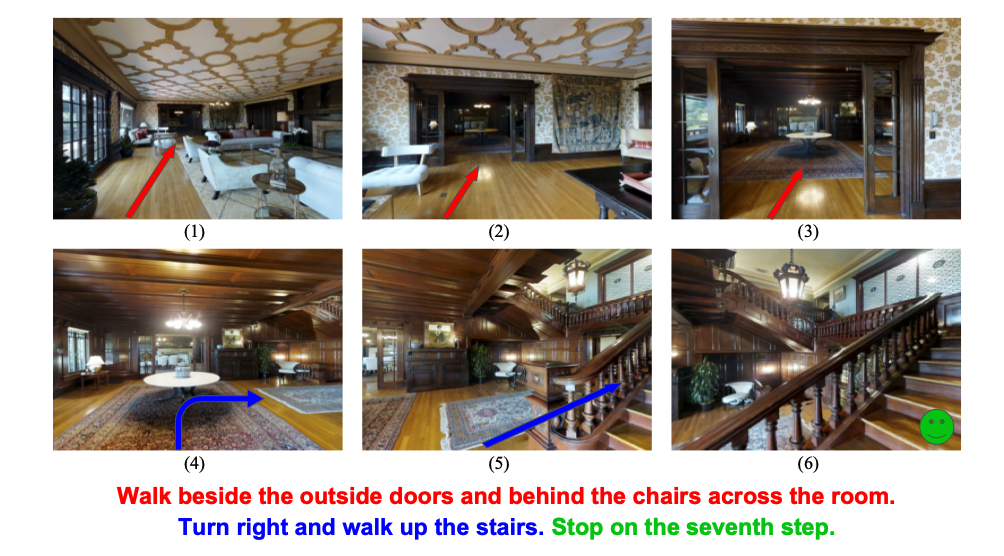
\includegraphics[height=5cm]{figures/r2r}
        \caption{The Room-to-Room dataset [Anderson+ 2018]}
    \end{figure}
\end{frame}

\begin{frame}
    {Robot learning}
    \begin{figure}
        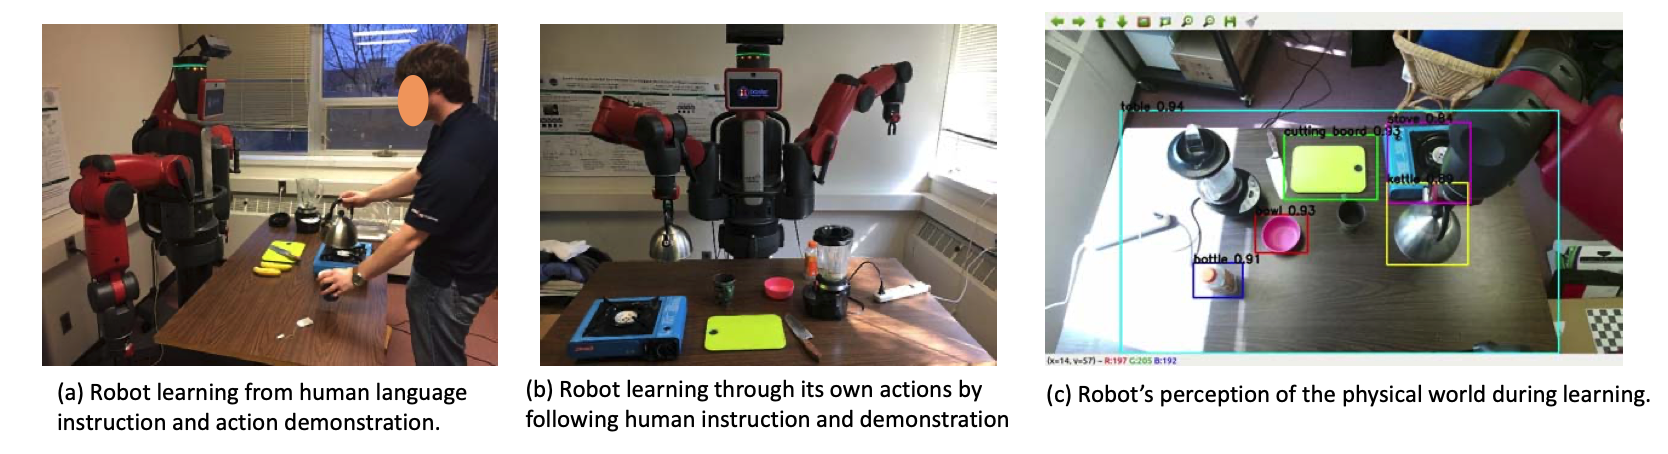
\includegraphics[height=3cm]{figures/robot-rl}
        \caption{ Interactive Task Learning with Physical Agents [Chai+ 2018]}
    \end{figure}

    Often require additional supervision: human demonstration, guidance through conversation
\end{frame}

\begin{frame}
    {Summary}
    Robot navigation with instructions

    Modeling: multimodal neural networks

    Learning: reinforcement learning (+ supervised learning)\\
    \begin{itemize}
        \item Learn the connection between language and the world in an end-to-end way
        \item Require a large number of interactions (may not be realistic)
    \end{itemize}

    Inference: best action (+ planning)
\end{frame}

\subsection{Speaker-listener models (adapted from Chris Potts' slides)}
\begin{frame}
    {Speakers and listeners}
    Speakers: world to language\\
    \begin{itemize}
        \item Image caption
        \item Color description
        \item Instruction giving
    \end{itemize}

    Listeners: language to world\\
    \begin{itemize}
        \item Semantic parsing
        \item Visual reasoning
        \item Instruction following
    \end{itemize}

    What are scenarios/tasks with both listeners and speakers?
\end{frame}

\begin{frame}
    {Reference games}
    Identify the target image
    \begin{figure}
        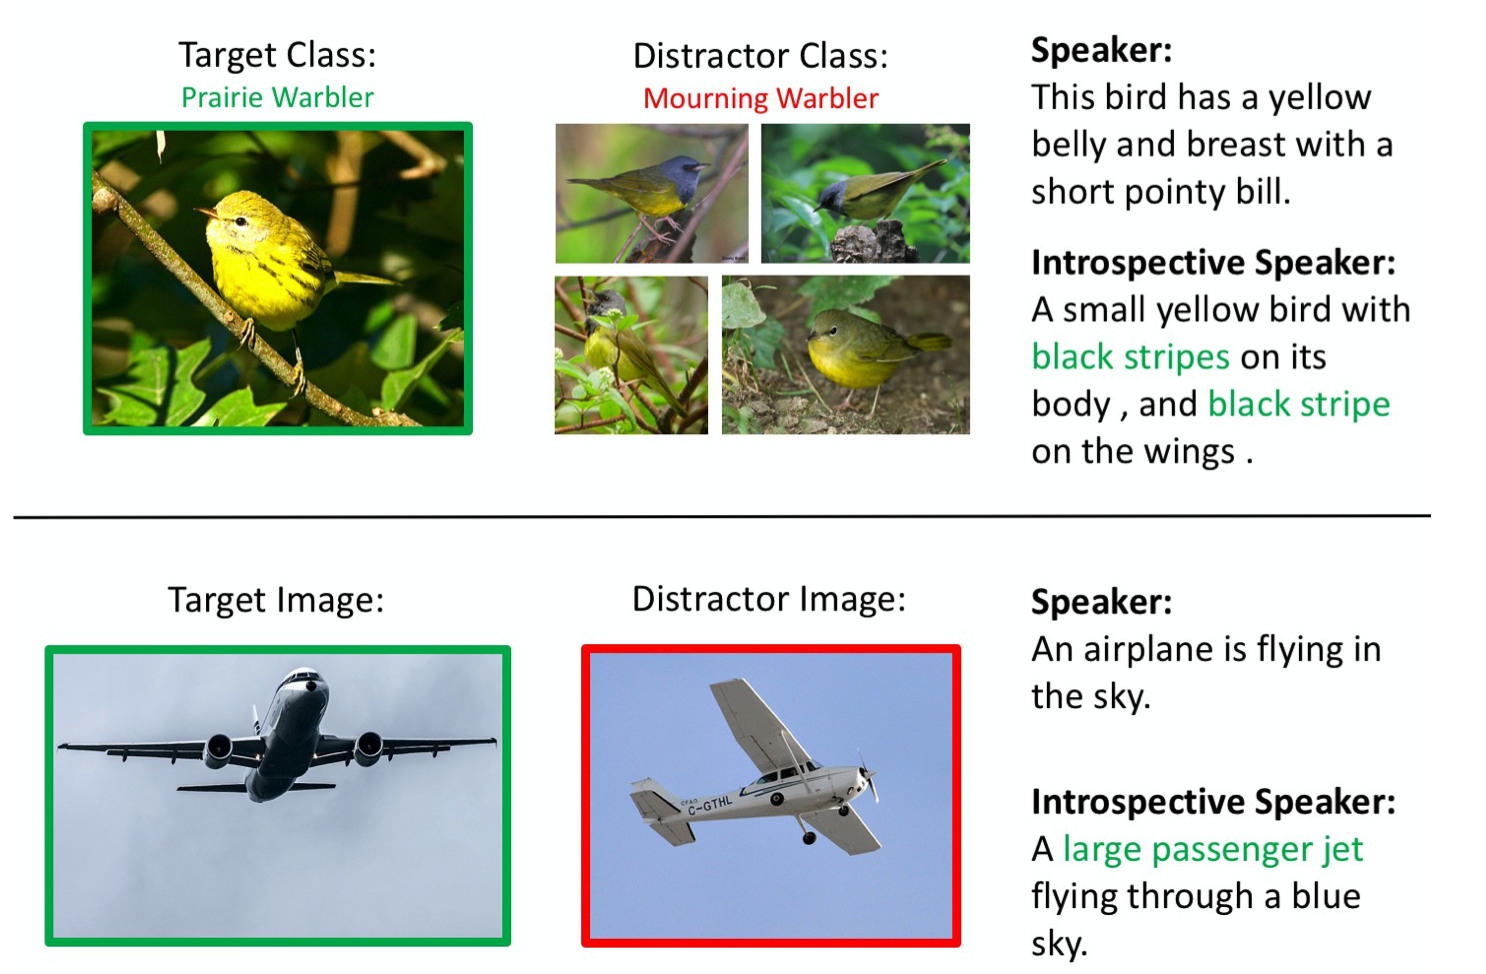
\includegraphics[height=5cm]{figures/dis-caption}
        \caption{[Vedantam+ 2017]}
    \end{figure}
    \vspace{-1em}
    \begin{itemize}
        \item Base speaker: caption is consistent with both images
        \item Context-sensitive speaker: caption is discriminative
    \end{itemize}
\end{frame}

\begin{frame}
    {Generating and following instructions}
    \begin{figure}
        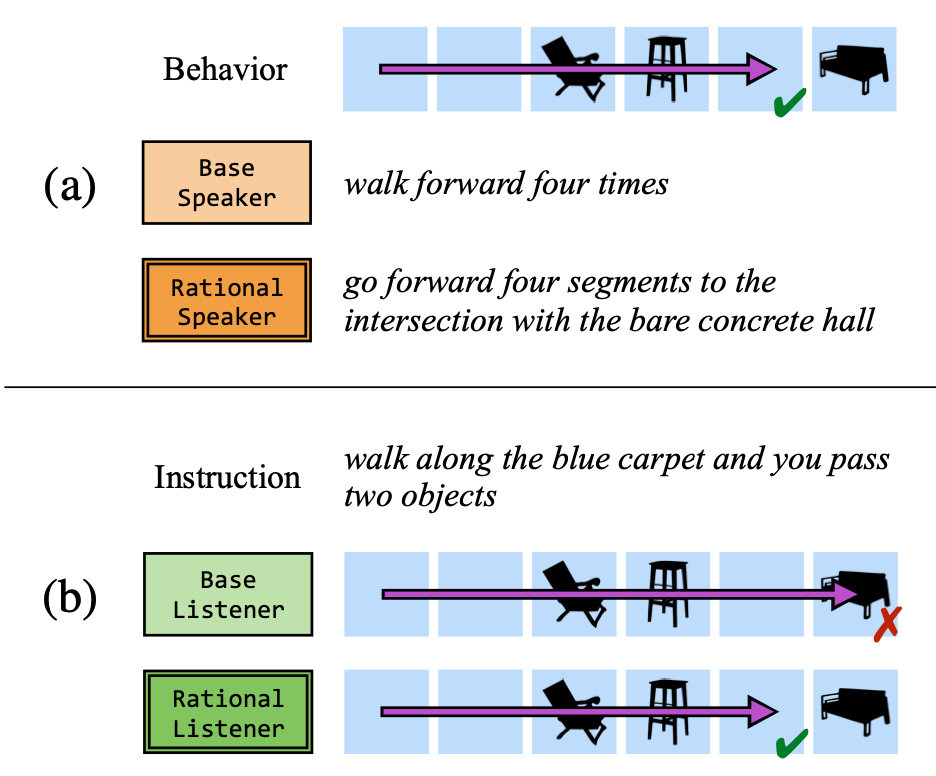
\includegraphics[height=5cm]{figures/ins-gen-follow}
        \caption{[Fried+ 2018]}
    \end{figure}
    \vspace{-1em}
    \begin{itemize}
        \item Rational speaker: what's the listener's orientation?
        \item Rational listener: should I pass exactly two objects or at least two? 
    \end{itemize}
\end{frame}

\begin{frame}
    {Collaborative games}
    \begin{figure}
        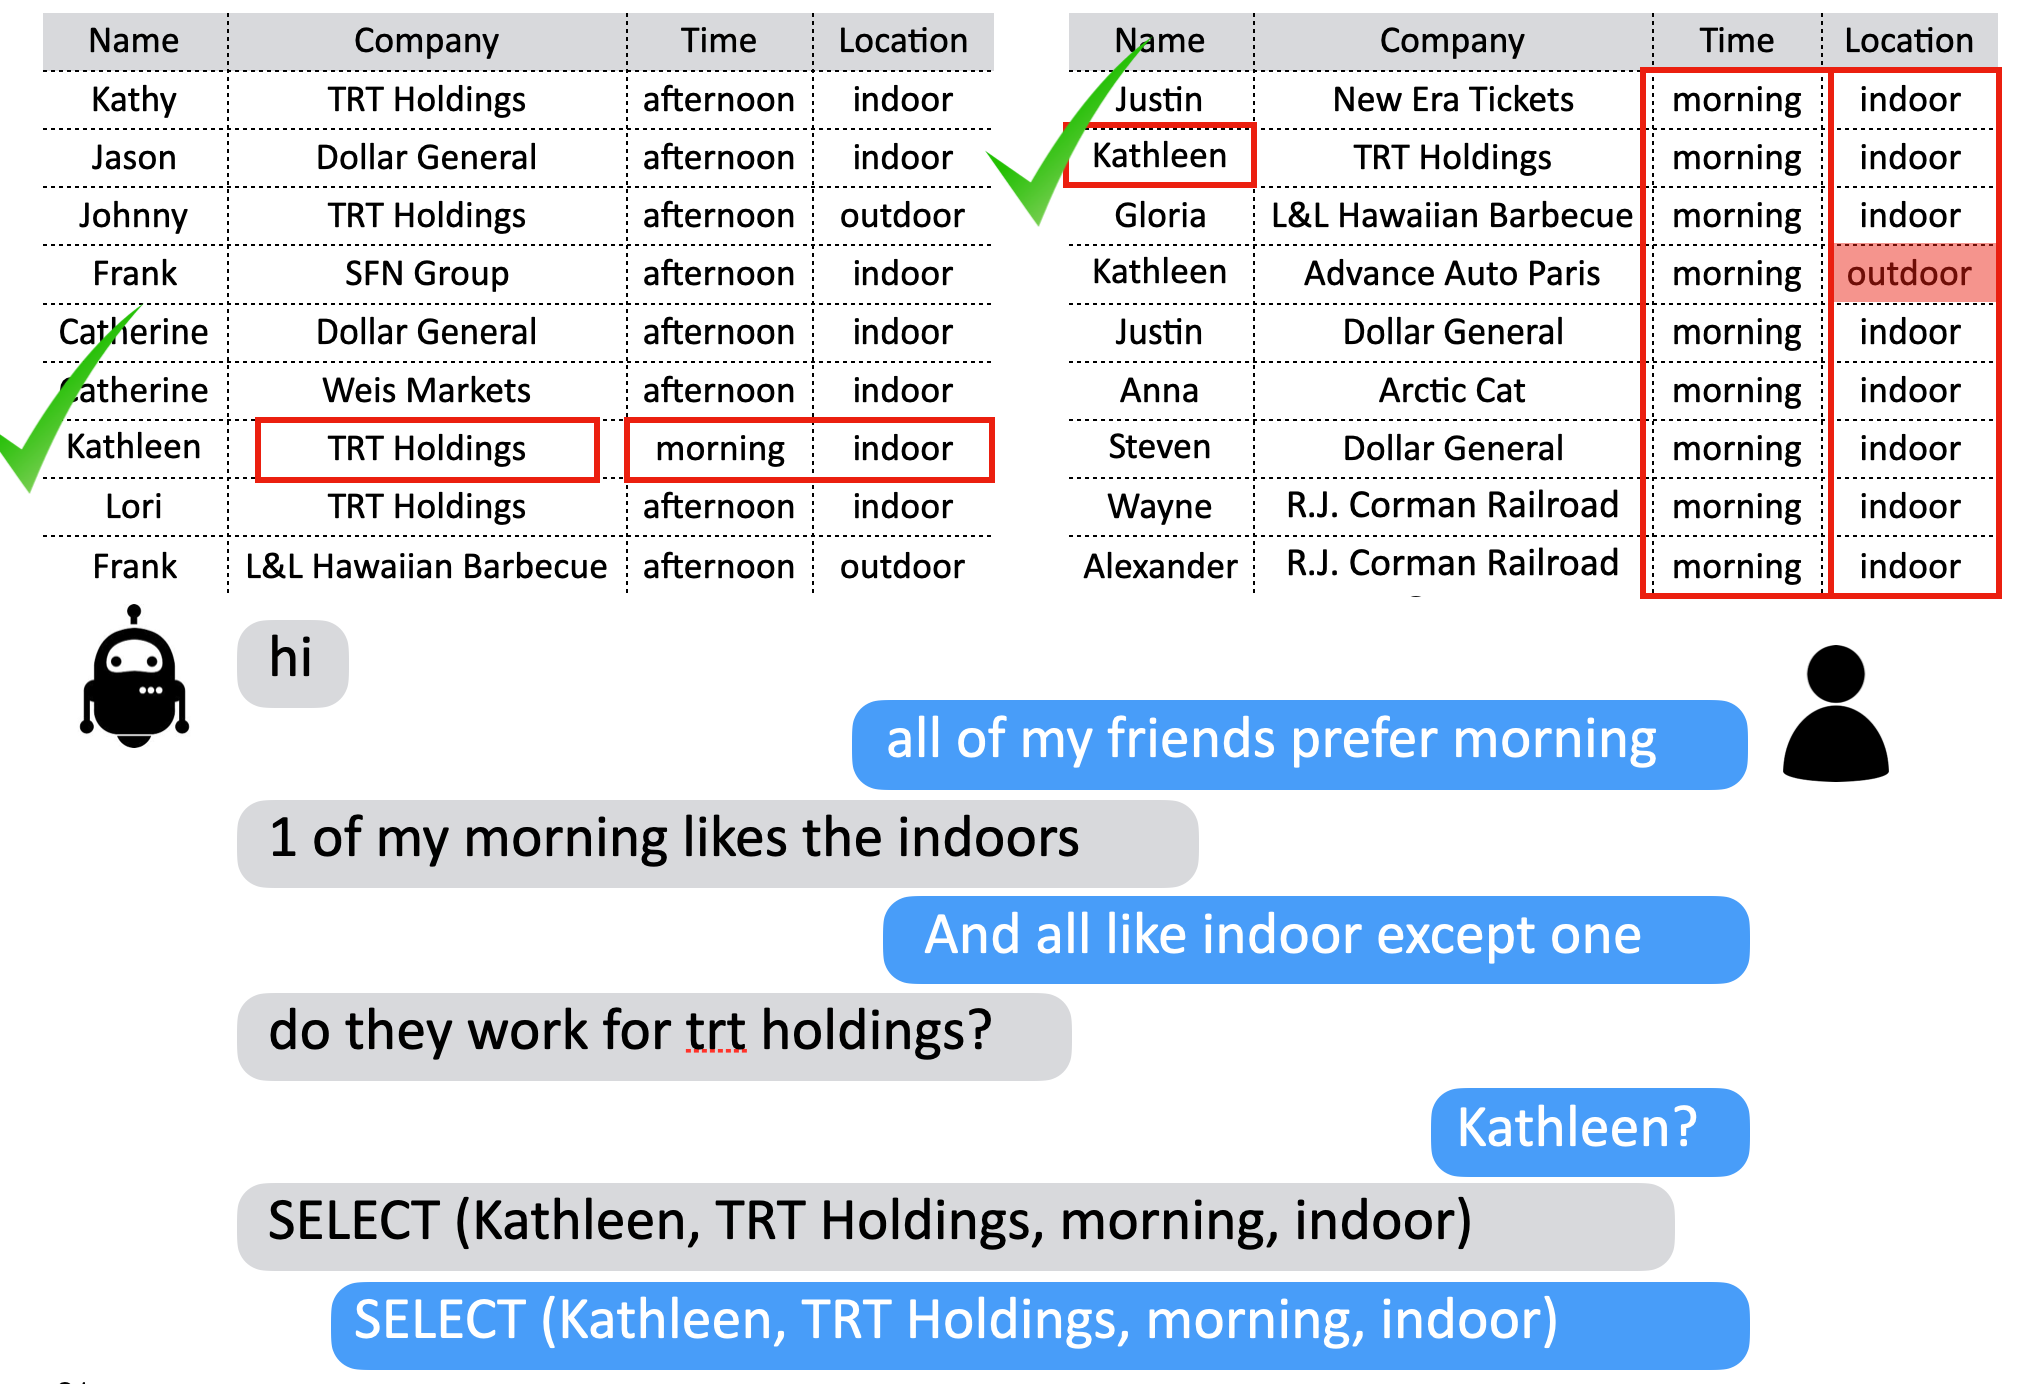
\includegraphics[height=5cm]{figures/mutualfriends}
        \caption{[He+ 2017]}
    \end{figure}
    \begin{itemize}
        \item Need knowledge from both agents to solve the puzzle
        \item Efficient collaboration requires reasoning about the other agent's knowledge 
    \end{itemize}
\end{frame}

\begin{frame}
    {Efficient referential communication}
    \begin{center}
    \begin{tikzpicture}
        \node (a) [rectangle,fill=blue!40!white,minimum size=1cm] at(0,0) {};
        \node (b) [circle,fill=blue!40!white,minimum height=1cm,right=1cm of a] {};
        \node (c) [rectangle,fill=green!40!white,minimum size=1cm,right=1cm of b] {};
    \end{tikzpicture}
    \end{center}

    $\text{state} = \pc{ \text{blueSquare}, \text{blueCircle}, \text{greenSquare} }$

    $\text{utterance} = \pc{\text{square}, \text{circle}, \text{green}, \text{blue}}$

    Assuming the speaker is cooperative, which object does ``blue'' refer to?
\end{frame}

\begin{frame}
    {Rational speech act model}
    \begin{center}
    \begin{tikzpicture}
        \node (a) [rectangle,fill=blue!40!white,minimum size=1cm] at(0,0) {};
        \node (b) [circle,fill=blue!40!white,minimum height=1cm,right=1cm of a] {};
        \node (c) [rectangle,fill=green!40!white,minimum size=1cm,right=1cm of b] {};
    \end{tikzpicture}
    \end{center}
    \textbf{Literal listener}: interprets an utterance according to its literal meaning\\
    \hspace{2em} ``blue'': blueSquare or blueCircle

    \textbf{Pragmatic speaker}: minimize the literal listener's effort of inferring the state while maximizing communication efficiency\\
    \hspace{2em} blueSquare: ``blue'' or ``square''

    \textbf{Pragmatic listener}: infer the state by reasoning about the pragmatic speaker\\
    \hspace{2em} ``blue'': blueSquare
\end{frame}

\begin{frame}
    {Rational speech act model}
    \begin{center}
    \begin{tikzpicture}
        \node (a) [rectangle,fill=blue!40!white,minimum size=1cm] at(0,0) {};
        \node (b) [circle,fill=blue!40!white,minimum height=1cm,right=1cm of a] {};
        \node (c) [rectangle,fill=green!40!white,minimum size=1cm,right=1cm of b] {};
    \end{tikzpicture}

        \begin{tabular}{cp{2cm}p{2cm}p{2cm}}
        blue & 1/2 & 1/2 & 0 \\
        square & 1/2 & 0 & 1/2 \\
        circle & 0 & 1 & 0 \\
        green & 0 & 0 & 1
        \end{tabular}
    \end{center}
    \textbf{Literal listener $L_0$}: interprets an utterance according to its literal meaning
    $$
    p_{L_0}(s\mid u) \propto \underbrace{p(s)}_{\text{state prior}}
    \underbrace{m(s,u)}_{\text{world model}}
    $$
\end{frame}

\begin{frame}
    {Rational speech act model}
    \begin{center}
    \begin{tikzpicture}
        \node (a) [rectangle,fill=blue!40!white,minimum size=1cm] at(0,0) {};
        \node (b) [circle,fill=blue!40!white,minimum height=1cm,right=1cm of a] {};
        \node (c) [rectangle,fill=green!40!white,minimum size=1cm,right=1cm of b] {};
    \end{tikzpicture}
        \begin{tabular}{cp{2cm}p{2cm}p{2cm}}
        blue   & 1/2 & 1/3   & 0 \\
        square & 1/2 & 0     & 1/3 \\
        circle & 0   & 2/3   & 0 \\
        green  & 0   & 0     & 2/3
        \end{tabular}
    \end{center}
    \textbf{Pragmatic speaker}: minimize the literal listener's effort of inferring the state while maximizing communication efficiency
    \begin{align*}
        p_{S_1}(u\mid s) &\propto \exp(\alpha U_{S_1}(u; s)) \\
        U_{S_1}(u; s) &= \log p_{L_0}(s\mid u) - C(u)
    \end{align*}
\end{frame}

\begin{frame}
    {Rational speech act model}
    \begin{center}
    \begin{tikzpicture}
        \node (a) [rectangle,fill=blue!40!white,minimum size=1cm] at(0,0) {};
        \node (b) [circle,fill=blue!40!white,minimum height=1cm,right=1cm of a] {};
        \node (c) [rectangle,fill=green!40!white,minimum size=1cm,right=1cm of b] {};
    \end{tikzpicture}
        \begin{tabular}{cp{2cm}p{2cm}p{2cm}}
        blue   & 3/5 & 2/5   & 0 \\
        square & 3/5 & 0     & 2/5 \\
        circle & 0   & 1   & 0 \\
        green  & 0   & 0     & 1 
        \end{tabular}
    \end{center}
    \textbf{Pragmatic listener}: infer the state by reasoning about the pragmatic speaker
    \begin{align*}
        p_{L_1}(s\mid u) &\propto p_{S_1}(u\mid s)p(s) \\
    \end{align*}
\end{frame}

\begin{frame}
    {Neural RSA}
    Limitation of RSA\\
    \begin{itemize}
        \item Pre-defined (small) lexicon
        \item Enumerate over all possible sequences
    \end{itemize}

    Learned speaker and listener with basic reasoning \mycite{[Andreas+ 2016]}
    \begin{tikzpicture}
        \node (a) [anchor=east]{
            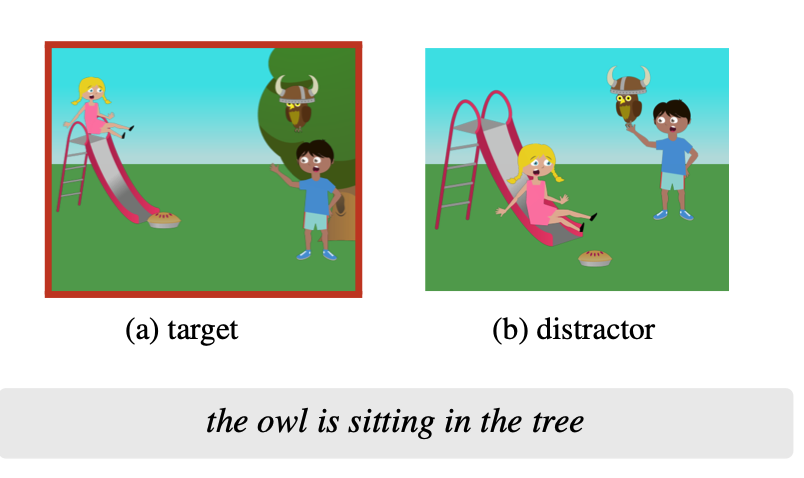
\includegraphics[height=3cm]{figures/neural-rsa-1}
        };
        \node (b) [right=1cm of a] {
            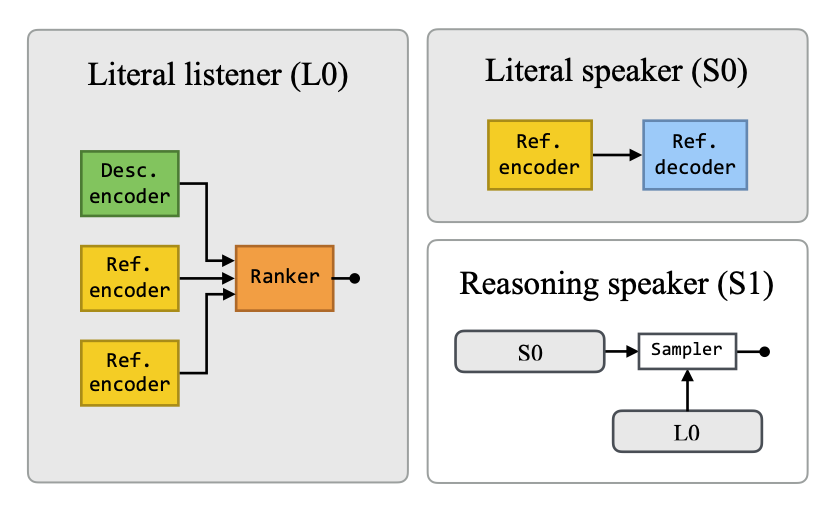
\includegraphics[height=3cm]{figures/neural-rsa-2}
        };
    \end{tikzpicture}
\end{frame}

\begin{frame}
    {Summary}
    \begin{itemize}
        \item Philosophy: language as a tool
        \item Goal: build agents with language capability working in human-centered environments
        \item Challenge: scale to realistic, persistent, interactive scenarios (with humans)
    \end{itemize}
\end{frame}

\end{document}
